\documentclass{article}
\usepackage[utf8]{inputenc}
\usepackage{tikz}
\usetikzlibrary{shapes,arrows,positioning}
\usepackage{hyperref}

\title{FreeCAD FEM Workbench Documentation}
\author{FreeCAD Community}
\date{\today}

\begin{document}

\maketitle
\tableofcontents

\section{Introduction}
This document provides an overview of the FreeCAD FEM Workbench, focusing on the integration between the Keyword Editor, Nodeset Extractor, and Solver components.

\section{System Architecture}

\begin{figure}[h]
\centering
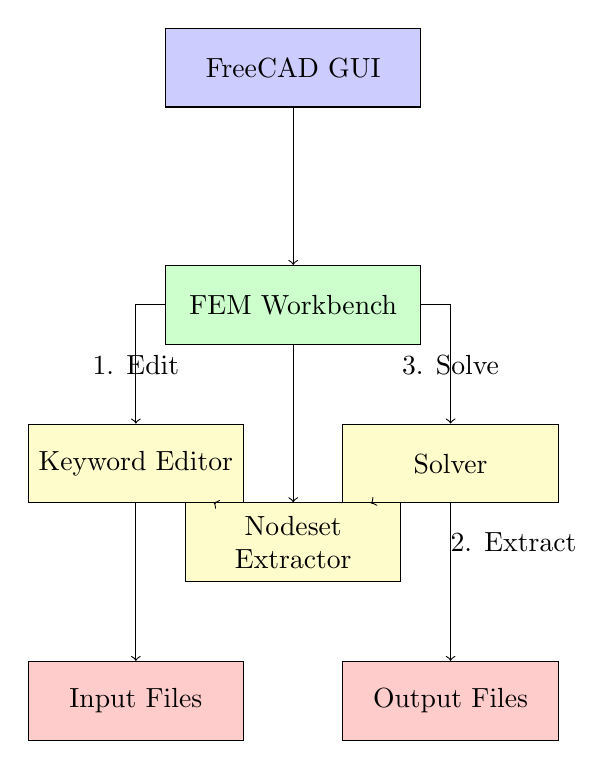
\begin{tikzpicture}[node distance=2cm, auto]
    % Nodes
    \node (gui) [rectangle, draw, fill=blue!20, text width=3cm, text centered, minimum height=1cm] {FreeCAD GUI};
    
    \node (femwb) [rectangle, draw, fill=green!20, text width=3cm, text centered, minimum height=1cm, below=of gui] {FEM Workbench};
    
    \node (ke) [rectangle, draw, fill=yellow!20, text width=2.5cm, text centered, minimum height=1cm, below left=1cm and -1cm of femwb] {Keyword Editor};
    \node (ne) [rectangle, draw, fill=yellow!20, text width=2.5cm, text centered, minimum height=1cm, below=of femwb] {Nodeset Extractor};
    \node (solver) [rectangle, draw, fill=yellow!20, text width=2.5cm, text centered, minimum height=1cm, below right=1cm and -1cm of femwb] {Solver};
    
    \node (input) [rectangle, draw, fill=red!20, text width=2.5cm, text centered, minimum height=1cm, below=of ke] {Input Files};
    \node (output) [rectangle, draw, fill=red!20, text width=2.5cm, text centered, minimum height=1cm, below=of solver] {Output Files};
    
    % Arrows
    \draw [->] (gui) -- (femwb);
    \draw [->] (femwb) -| (ke);
    \draw [->] (femwb) -- (ne);
    \draw [->] (femwb) -| (solver);
    \draw [->] (ke) -- (ne);
    \draw [->] (ne) -- (solver);
    \draw [->] (ke) -- (input);
    \draw [->] (solver) -- (output);
    
    % Labels
    \node [above=0.5cm of ke] {1. Edit};
    \node [right=0.5cm of ne] {2. Extract};
    \node [above=0.5cm of solver] {3. Solve};
\end{tikzpicture}
\caption{Top-down flow of the FEM Workbench}
\label{fig:flow}
\end{figure}

\section{Key Components}

\subsection{Keyword Editor}
The Keyword Editor allows users to:
\begin{itemize}
    \item Edit solver-specific keywords and parameters
    \item Validate input files before execution
    \item Save and load solver configurations
    \item Support for multiple solvers (CalculiX, OpenRadioss, etc.)
\end{itemize}

\subsection{Nodeset Extractor}
The Nodeset Extractor provides:
\begin{itemize}
    \item Automatic node set creation from geometry
    \item Support for various constraint types (force, displacement, etc.)
    \item Visualization of node sets
    \item Export/import capabilities
\end{itemize}

\subsection{Solver Integration}
The Solver component handles:
\begin{itemize}
    \item Execution of analysis
    \begin{itemize}
        \item Input file processing
        \item Output directory management
    \end{itemize}
    \item Progress monitoring
    \item Error handling and logging
\end{itemize}

\section{Workflow}

\subsection{1. Model Setup}
\begin{enumerate}
    \item Create or import geometry
    \item Define material properties
    \item Apply boundary conditions
\end{enumerate}

\subsection{2. Nodeset Extraction}
\begin{enumerate}
    \item Select geometry for node sets
    \item Extract nodes using the Nodeset Extractor
    \item Verify node sets in the 3D view
\end{enumerate}

\subsection{3. Solver Configuration}
\begin{enumerate}
    \item Open the Keyword Editor
    \item Configure solver parameters
    \item Save the input file
\end{enumerate}

\subsection{4. Execution}
\begin{enumerate}
    \item Run the solver
    \item Monitor progress
    \item View results
\end{enumerate}

\section{Example}

\begin{verbatim}
# Example Python API usage
import FreeCAD
from femutils.nodeset_extractor import extract_nodesets

# Get the active document
doc = FreeCAD.ActiveDocument

# Extract nodesets from analysis
analysis = doc.Analysis
mesh_obj = doc.Mesh
nodesets = extract_nodesets(analysis, mesh_obj)

# Print extracted nodesets
for name, nodes in nodesets.items():
    print(f"{name}: {nodes}")
\end{verbatim}

\end{document}
